% Options for packages loaded elsewhere
\PassOptionsToPackage{unicode}{hyperref}
\PassOptionsToPackage{dvipsnames,svgnames*,x11names*}{xcolor}

% Set document class options
\documentclass[webpdf,large,contemporary,namedate]{oup-authoring-template}

% one column
\onecolumn

%\usepackage{showframe}

% line numbers

% use upquote if available, for straight quotes in verbatim environments
\IfFileExists{upquote.sty}{\usepackage{upquote}}{}

% From Pandoc template for its feature
\usepackage{xcolor}
\usepackage{hyperref}

\hypersetup{
  pdftitle={Incorporating varying degrees of spatial cohesion in models of voter behaviour in the UK General Election 2024},
  pdfkeywords={elections, ICAR modelling, spatial cohesion, spatial
regression},
  breaklinks=true,
  bookmarks=true,
  colorlinks=true,
  linkcolor={Maroon},
  filecolor={Maroon},
  citecolor={Blue},
  urlcolor={orange},
  pdfcreator={LaTeX via pandoc}}



% tightlist command for lists without linebreak
\providecommand{\tightlist}{%
  \setlength{\itemsep}{0pt}\setlength{\parskip}{0pt}}




% Counters for addresses and footnotes
\newcounter{correspcnt} % For author footnotes
\renewcommand*{\thecorrespcnt}{\fnsymbol{correspcnt}}
\newcounter{addrcnt} % For author addresses

% Macros for dealing with affiliations, footnotes, etc.
\makeatletter

\def\MyNewLabel#1#2#3{\expandafter\gdef\csname #1@#2\endcsname{#3}}

\def\MyRef#1#2{\@ifundefined{#1@#2}{???}{\csname #1@#2\endcsname}}

\newcommand*\ifcounter[1]{%
  \ifcsname c@#1\endcsname
    \expandafter\@firstoftwo
  \else
    \expandafter\@secondoftwo
  \fi
}

\newcommand*\addrlblbycode[1]{%
  \ifcounter{ADDRLBL@#1}
    {}
    {\refstepcounter{addrcnt}\newcounter{ADDRLBL@#1}\setcounter{ADDRLBL@#1}{\value{addrcnt}}}%
    \arabic{ADDRLBL@#1}%
}

\newcommand*\addrbycode[1]{%
  \ifcounter{ADDR@#1}
    {}
    {\newcounter{ADDR@#1}%
     \address[\addrlblbycode{#1}]{\MyRef{ADDRTXT}{#1}}}%
}

\newcommand*\corresplblbycode[1]{%
  \ifcounter{CORRESPLBL@#1}
    {}
    {\refstepcounter{correspcnt}\newcounter{CORRESPLBL@#1}\setcounter{CORRESPLBL@#1}{\value{correspcnt}}}%
    \fnsymbol{CORRESPLBL@#1}%
}

\newcommand*\correspbycode[1]{%
  \ifcounter{CORRESP@#1}
    {}
    {\newcounter{CORRESP@#1}%
     \corresp[\corresplblbycode{#1}]{\MyRef{CORRESPTXT}{#1}}}%
}

\makeatother

% Add missing \city command mentioned in documentation but absent from cls
\providecommand\city[1]{#1}

% Create labels for Addresses if the are given in Elsevier format
   \MyNewLabel{ADDRTXT}{ABC}{%
  %
  \orgdiv{Hamilton Institute}, %
  \orgname{Maynooth University}, %
  \orgaddress{%
   %
  %
  %
  \city{Maynooth}, %
  %
  \country{Ireland}%
  }%
   %
 %
 }
   \MyNewLabel{ADDRTXT}{DEF}{%
  Department of Mathematics and Statistics, Maynooth University,
Maynooth, Ireland%
 }
   \MyNewLabel{ADDRTXT}{GHI}{%
  National Centre for Geocomputation, Maynooth University, Maynooth,
Ireland%
 }

% Create labels for Footnotes if they are given in Elsevier format

% Pandoc header-include feature
\theoremstyle{thmstyleone}
\newtheorem{theorem}{Theorem}
\newtheorem{proposition}[theorem]{Proposition}
\theoremstyle{thmstyletwo}
\newtheorem{example}{Example}
\newtheorem{remark}{Remark}
\theoremstyle{thmstylethree}
\newtheorem{definition}{Definition}
\renewcommand\normalsize{\fontsize{10}{12}\selectfont}
\normalsize
\usepackage[font=normalsize]{caption}
% Pandoc header-include feature
\usepackage{booktabs}
\usepackage{longtable}
\usepackage{array}
\usepackage{multirow}
\usepackage{wrapfig}
\usepackage{float}
\usepackage{colortbl}
\usepackage{pdflscape}
\usepackage{tabu}
\usepackage{threeparttable}
\usepackage{threeparttablex}
\usepackage[normalem]{ulem}
\usepackage{makecell}
\usepackage{xcolor}

\begin{document}

\journaltitle{Journal Name}
\DOI{DOI HERE}
\copyrightyear{YYYY}
\pubyear{YYYY}
\access{Advance Access Publication Date: Day Month Year}
\appnotes{Paper}

\firstpage{1}



\title[]{Incorporating varying degrees of spatial cohesion in models of
voter behaviour in the UK General Election 2024}

\newcounter{thisauthcorresp} % For storage if author is corresponding author
\newcounter{thisauththanks} % For storage if author has thanks



\author[%
\addrlblbycode{ABC}%
,\refstepcounter{correspcnt}\setcounter{thisauthcorresp}{\value{correspcnt}}\fnsymbol{thisauthcorresp}%
%
%
]{Kevin Horan}

\addrbycode{ABC}

\corresp[\fnsymbol{thisauthcorresp}]{Corresponding author. \href{mailto:kevin.horan.2021@mumail.ie}{\nolinkurl{kevin.horan.2021@mumail.ie}}}




\author[%
\addrlblbycode{DEF}%
%
%
%
]{Katarina Domijan}

\addrbycode{DEF}






\author[%
\addrlblbycode{GHI}%
%
%
%
]{Chris Brunsdon}

\addrbycode{GHI}






% Add author mark
\authormark{Kevin Horan et al.}

\received{Date}{0}{Year}
\revised{Date}{0}{Year}
\accepted{Date}{0}{Year}

%\editor{Associate Editor: Name}

\abstract{
Fitting models to data where multiple spatial processes are assumed to
be operating simultaneously at different levels is often done by
combining a hierarchical effects structure at the higher levels (region,
county) with autoregressive structures at the lowest (individual data
points). When dealing with areal data, an intrinsic conditional
autoregressive (ICAR) component is often used to capture these lowest
level spillover effects. One of the standard assumptions of ICAR models
is a global spatial variance parameter, meaning all areas undergo the
same degree of smoothing. We propose allowing this variance parameter to
change, reflecting different degrees of spatial cohesion in different
regions. We demonstrate an application using voter behaviour in the 2024
UK General Election. This technique has not enjoyed widespread exposure,
particularly as regards election data. By fitting a series of models
representing different hypothesised spatial processes for the vote count
of each of the four largest parties and comparing the resultant marginal
likelihoods, we find that this novel approach is the most plausible
model, and reveals different patterns of spatial cohesion among the
parties.}

\keywords{elections; ICAR modelling; spatial cohesion; spatial
regression}


\maketitle


\section{Introduction}\label{introduction}

When modelling spatial data, it is well understood that there is a
tendency for nearby data points to be more similar than distant ones. It
is also possible that groups of these data points can be seen as
comprising regions, where a certain difference between and similarity
within region is to be expected. Each of these phenomena describes a
different type of spatial process, occurring at a different level of
data aggregation. The practice of incorporating both of these processes
simultaneously in a model has been termed hierarchical spatial
autoregressive modelling (HSAM) by \citet{dong2015}. They describe this
as analogous to a combination of vertical and horizontal spatial
processes.

The vertical processes can be captured using hierarchical modelling
structures \citep{goldstein1997}. When applied in a geographical
context, where the levels might refer to administrative units such as
regions and counties \citep{jones1991}, this top-down structure
positions a spatial unit within a tree structure (e.g.~a location in a
town which lies within a province within a country). While this can do a
good job at grouping potentially similar places together and sharing
information across such groups, it can still lead to a situation where
the potential relationship between neighbouring data points which happen
to lie on either side of an administrative boundary is ignored.

The horizontal process can capture such neighbourhood relationships,
regardless of group boundaries. This relies on an autoregressive
structure to model spillover effects where each data point is dependent
on nearby data points. Spatial units which are neighbours are expected
to share similarities. One commonly-used such structure in areal models
is an intrinsic conditional autoregressive (ICAR) component
\citep{besag1974} which contributes a set of spatially smoothed random
effects at the level of individual data points which are correlated
according to contiguity, with each unit's effect being Normally
distributed around the mean of that of its neighbours. The strength of
this smoothing is controlled by a single variance parameter for the
entire area.

Variations on this approach, particularly in the field of
disease-modelling, include the BYM model \citep{besag1991} which
combines this spatially structured component based on contiguity with an
additional unstructured effect (i.i.d. Gaussian), and the related BYM2
model \citep{Riebler2016} which further parametrises the structure with
a component to account for the relative proportion of each source of
variation.

We propose a technique which combines group structures and an
autoregressive component in a different way. Rather than capturing
higher level group differences with a set of random effects where each
group has a different mean divergence from the global mean, we instead
incorporate group variation in the ICAR process itself, by allowing the
variance parameter to vary by region, meaning that the strength of the
spatial smoothing differs across groups. For units within each region,
the random effect still depends on the average of the neighbours' random
effects, but the amount of random variation around this average is
determined by the group-specific variance parameter. Regions with lower
variance exhibit stronger spatial smoothing (smaller variability among
neighbours), while regions with higher variance allow for greater
heterogeneity in the random effects within that region. This allows us
to capture differences in spatial cohesion which may better account for
the process than region random effects.

There are other approaches to the idea of a non-stationary variance
component in the literature. \citet{Brewer2007} introduced edge-specific
weights within the contiguity structure to enable locally varying
smoothness between all pairs of units. An iterative algorithm was
proposed by \citet{DuncanLee2014} to detect spatial discontinuities and
update the adjacency structure itself. \citet{Jack2019} used a
spatio-temporal model where the degree of spatial cohesion could vary
with time. However, these methods do not seek to incorporate a
hypothesised hierarchical structure within the ICAR variance parameter.

In this article, we examine an application of this approach using data
from the 2024 UK General Election to see if it proves more plausible
than other hypothesised approaches. Before discussing the spatial
processes which we will consider, we first mention some other factors
which are at play in the modelling of voting behaviour.

As \citet{griffiths2024brexit} point out, it is well known that
socio-economic factors - predominantly social class \citep{Butler1974},
education, age, deprivation and ethnicity - have long been strongly
associated with political preferences in the UK, although
\citet{Jennings2024} observe that both their strength and direction of
association have been changing over time for different parties.

In the coverage of this particular election, there was also a strong
narrative of potential tactical voting where a voter might choose which
party to vote for not based on a preference for that party but with the
aim of maximising the chances of unseating the incumbent. This is
particularly encouraged by the UK's first-past-the-post electoral
system. Although difficult to model explicitly, it is clearly connected
to the marginality and incumbency of a seat \citep{Muller2015}. The size
of the lead held by an incumbent party, whether or not that party is
currently in government, and the identity of its closest competitor
could all influence the likelihood of tactical voting occurring. By
controlling for the incumbent party in each constituency, and also the
second placed party from the previous election and the size of the
majority, we seek to capture trends which are consistent with this type
of behaviour.

Having controlled for these socio-economic and \emph{status quo ante}
factors, we still theorise that there would be unaccounted for spatial
processes at play in determining voter behaviour. There are a number of
reasons why voters might behave in a way which would reflect a vertical
regional structure. Different parts of the country have deep-rooted
political cultures associated with place and may be reluctant to change
from these. The regional scale has proven useful
\citep{pattie1995region} and can, for some contextual effects, be more
powerful than local scales \citep{Pattie2013}. Furthermore, policies
which a party proposes in a manifesto can have a spatial aspect to them
which can make them more or less appealing to voters in a particular
region. In the UK context, this could apply to ``levelling-up'', issues
regarding the green belt, energy policy etc.

We would also expect a horizontal neighbourhood component when modelling
voter behaviour. People who live nearby, work together, or associate
together in bars, clubs and other organisations have a tendency to align
in their political views, as summarised by \citet{pattie2000} in the
maxim ``those who speak together vote together'', referencing work done
by \citet{Miller1977}.

These two types of processes have been combined together in a HSAM
framework in the context of voting behaviour by \citet{Horan2024}, more
specifically, examining swing between Labour and Conservatives in the
2019 election.

In the following application, to avoid complications arising from
parties which competed only in Scotland, Wales and Northern Ireland, we
restrict the study area to England where this election saw increased
party system fragmentation \citep{Prosser2024} with the emergence of
four dominant parties (each receiving greater than 10\% of the national
vote and a combined total of almost 90\%): Labour, Conservatives,
Liberal Democrats and Reform UK (see Table \ref{tab:elecsummary}). We
aim to model the number of votes obtained by each party in each
constituency using a Bayesian approach. We propose a selection of
credible models and compare their plausibility using log marginal
likelihoods. Before turning to the 2024 election data, exploratory
simulations are carried out to examine whether this approach can
correctly identify known underlying model structures as being the most
plausible. For the election data, we first fit models with no explicitly
spatial component and examine their residuals. The presence of residual
spatial patterns justifies the subsequent modelling exercises. Seven
further models are then fitted for each of the four parties. These
models increase in complexity from those which contain only one spatial
process to others using a HSAM framework with combined processes. One
such model is our novel approach allowing the variance of the ICAR
structure to change by region. We are then in a position to be able to
rank these models according to marginal likelihood and determine which
is most plausible for each party, given the voting data. In our example,
we find that the novel approach is the best model for all four parties,
revealing different patterns of spatial cohesion for each.

The utility of this model is not only that it seems to provide a more
plausible mechanism than other models in some circumstances. The set of
variance parameters which it estimates are of interest in their own
right as a measure of the degree to which nearby places tend to be
similar. Their interpretation will vary depending on the field of study,
but they offer an additional avenue of investigation for spatial
processes.

\section{Data}\label{data}

\subsection{Election 2024}\label{election-2024}

The 2024 UK General Election saw Labour defeat the incumbent
Conservative government. In England, the focus of this model, Labour
increased their seat count by 166, the Conservatives lost 229 seats, the
Liberal Democrats increased their seat count by 59, while Reform UK won
5 seats. However, owing to the first-past-the-post electoral system,
these numbers are far from reflective of the relative number of votes
cast for each party, particularly so in this election
\citep{Pattie2024}. Summaries of these seat and vote counts for each
party are shown in Table \ref{tab:elecsummary}. Despite winning only a
fraction of the number of seats which the Liberal Democrats attained,
Reform UK actually acquired a greater number of votes across England.
This is a result of the voting system and its interplay with differences
in concentration and distribution of votes by location, emphasising the
particularly key role played by geography in UK elections. For the
purposes of this study, we are not concerned with whether or not parties
won a particular seat. Instead, we attempt the model the total number of
votes gained by a party in each constituency.

The two data sources in this study are the 2021 census and the results
of the 2024 and 2019 General Elections. Census results were sourced from
the \citet{census2021} and voting data from the \citet{elections_data}.
The census results are available at the level of the 2024 constituency
boundaries so these were joined with the most recent election results.
When including results from the 2019 election as covariates, some
complications arose because of boundary changes. As a result, it has
been necessary for the purposes of comparison to re-project the 2019
constituency vote counts to their 2024 equivalents. This was achieved by
assigning 2019 constituency votes to 2024 constituencies according to
the proportion of population living in areas of overlap
\citep{boundary_changes}.\footnote{The conversion procedure is outlined
  in more detail at \url{https://github.com/horankev/voteReproject}.}

Of the 543 constituencies in England, 542 were considered. We omitted
Chorley as this was the constituency of the Speaker of the House which,
by convention, is not contested by the major parties. In subsequent
maps, it can be identified as an uncoloured unit towards the north west.
A Labour candidate competed in all 542 constituencies, a Conservative or
Liberal Democrat candidate in 541, and a Reform UK candidate in 521.

\begin{table*}

\caption{\label{tab:elecsummary}Percentage vote share, seat count, and percentage of seat totals in England for parties in the 2024 General Election. Four parties achieved a vote share greater than 10\%, totalling 89\% of the total votes cast and over 98\% of seats won.}
\centering
\fontsize{8}{10}\selectfont
\begin{tabular}[t]{l|r|r|r}
\hline
Party & Percentage of Votes & Seat Count & Percentage of Seats\\
\hline
Labour & 34.5 & 347 & 64.0\\
\hline
Conservative & 25.9 & 116 & 21.4\\
\hline
Reform UK & 15.4 & 5 & 0.9\\
\hline
Liberal Democrat & 13.2 & 65 & 12.0\\
\hline
Green & 7.3 & 4 & 0.7\\
\hline
Other & 3.7 & 5 & 0.9\\
\hline
\end{tabular}
\end{table*}

\subsection{Dependent variable}\label{dependent-variable}

The outcome we are seeking to model is vote count per constituency for
each party. To give an idea of the spatial patterns and variation
between parties, Figure \ref{fig:figvoteshare} shows the percentage of
votes which each party attained in 2024, diverging about the overall
median. We show percentages in this figure to control for different
constituencies having different populations. In these maps, the
constituencies are shown as hexagons of equal size, while still
approximating relative position. This overcomes the problem of
invisibility arising from some small, densely populated urban
constituencies. In later maps, where a more precise idea of relative
position and contiguity is an important consideration (as is the case
when exploring neighbourhood relationships) maps will be shown in
regular projection.

\begin{figure*}[th]
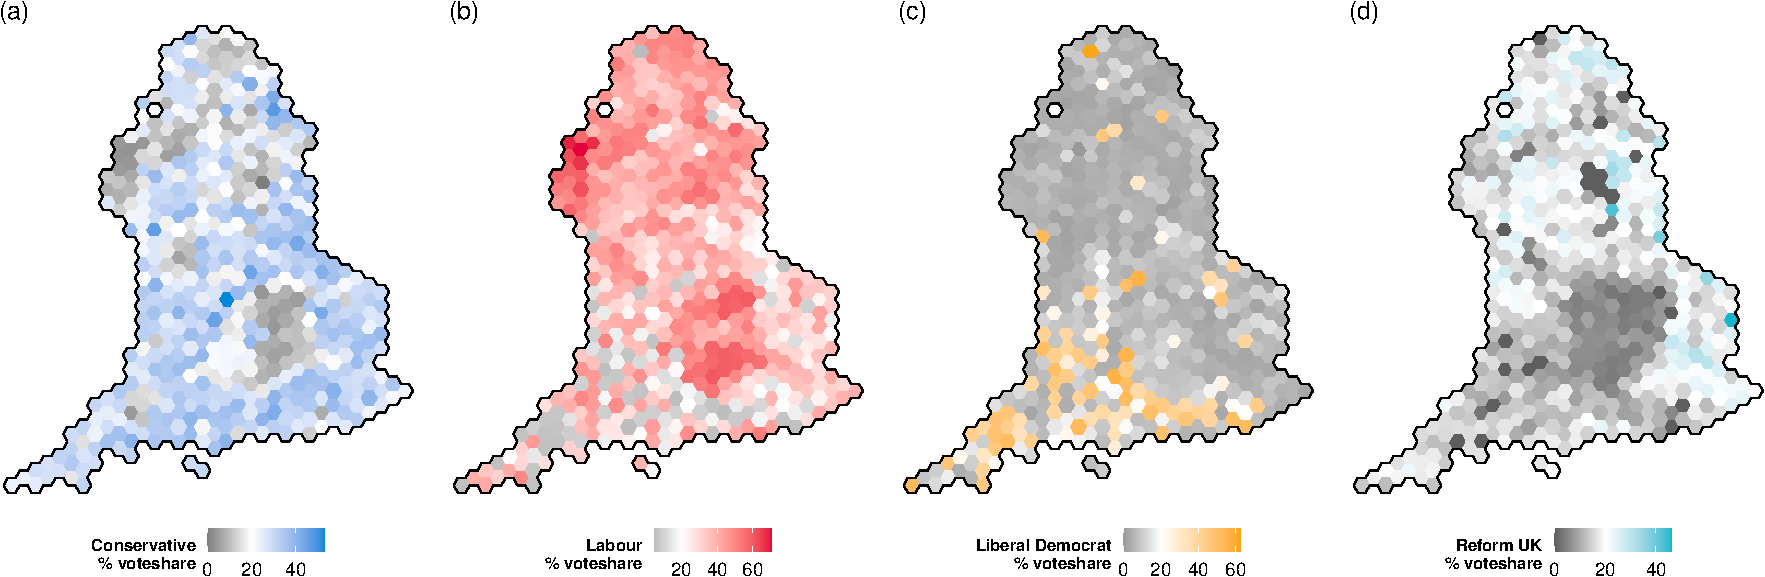
\includegraphics[width=1\linewidth]{jrss_resubmission3_files/figure-latex/figvoteshare-1} \caption{(a-d) Percentage vote share by constituency for four largest parties in 2024 UK General Election. The white hexagon towards the north west in these and subsequent maps represents the Speaker's seat which, by custom, is not contested.}\label{fig:figvoteshare}
\end{figure*}

\subsection{Explanatory variables}\label{explanatory-variables}

The three socio-economic variables included in the model from the 2021
census are shown in Figure \ref{fig:figsocec}, diverging about their
median values. They represent, respectively, the proportion of the
population of each constituency with a degree, the proportion
self-reporting fair, bad or very bad health, and the proportion of white
ethnicity. These three variables are a subset of those considered by
\citet{beecham2018} in a study of the connection between the narrative
of ``left-behind'' places and voting behaviour in the Brexit referendum.
Other variables which they considered included professional occupations,
younger adults, English as main language and home ownership. They were,
however, interested in examining individual relationships between these
variables and voting behaviour. As we are modelling these covariates
together, issues of multicollinearity would arise without careful
selection. These three variables were found to be highly correlated with
(and thus good proxies for) many other socio-demographic variables
(e.g.~degree education with professional occupations, poor health with
age, white with English-speaking, Christian and single-ethnicity
households), while also not leading to problematic levels of
multicollinearity, In the subsequent models, they are scaled to have a
mean of 0 and standard deviation of 1 to improve sampling efficiency and
stability in a Bayesian context.

\begin{figure*}[th]
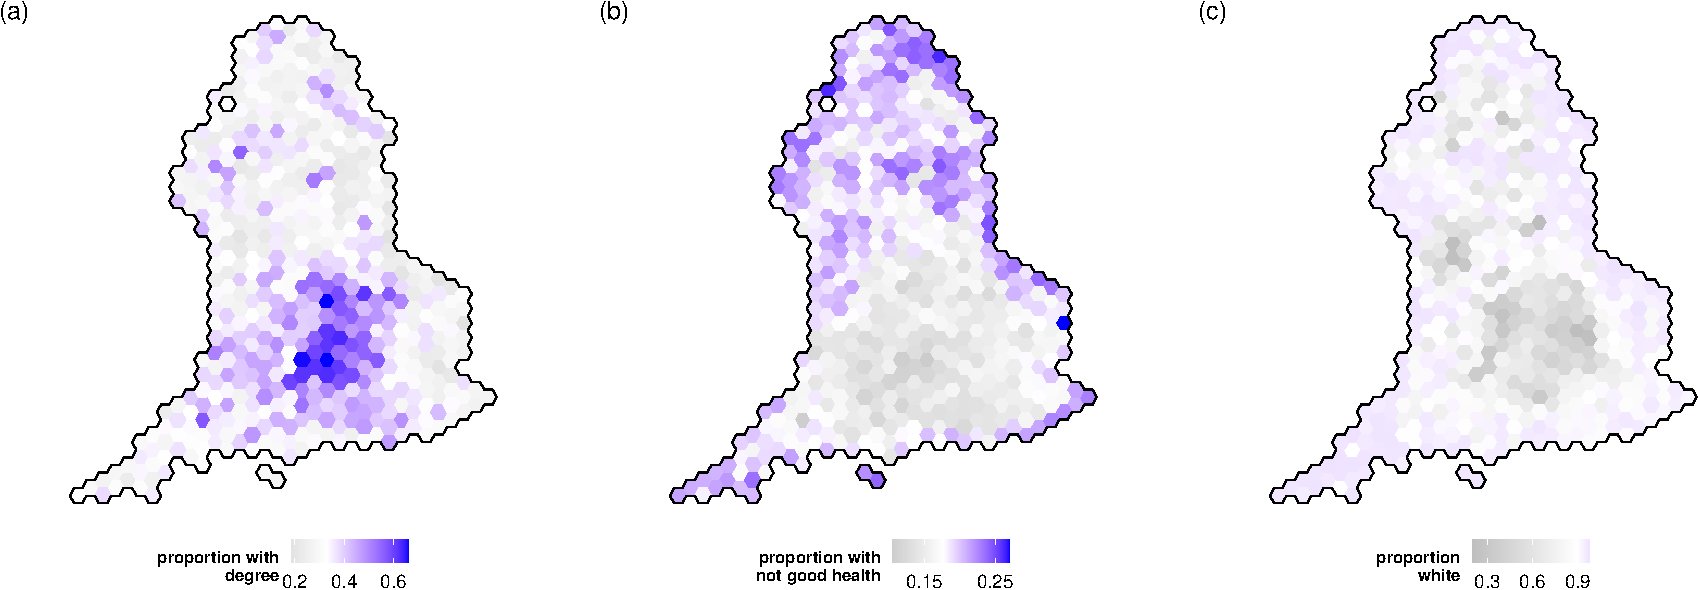
\includegraphics[width=1\linewidth]{jrss_resubmission3_files/figure-latex/figsocec-1} \caption{Proportion of population by constituency (a) with a degree, (b) with fair, bad or very bad health, and (c) of white ethnicity.}\label{fig:figsocec}
\end{figure*}

The model also accounts for potential drivers of tactical voting - the
winner and second placed party from the previous election, and the size
of the majority of the winning party, as shown in Figure
\ref{fig:figplacement}. This \emph{marginality} is calculated as the
difference between the total number of votes for the first and second
placed parties. Because of varying constituency size, it is expressed as
a proportion of the total overall number of votes cast in each
constituency. There is evidence that tactical voting tends to be higher
in marginal seats \citep{Cain1978tact, Johnston1992tact}. For the same
reasons as the socio-economic explanatory variables, these majorities
were also scaled.

While Reform UK are shown separately in the second place map in Figure
\ref{fig:figplacement} (c), they were the second placed party in only
one constituency in 2019. For this reason, they were included in the
\emph{other} category for this variable in the modelling process, along
with other parties and independent candidates.

\begin{figure*}[th]
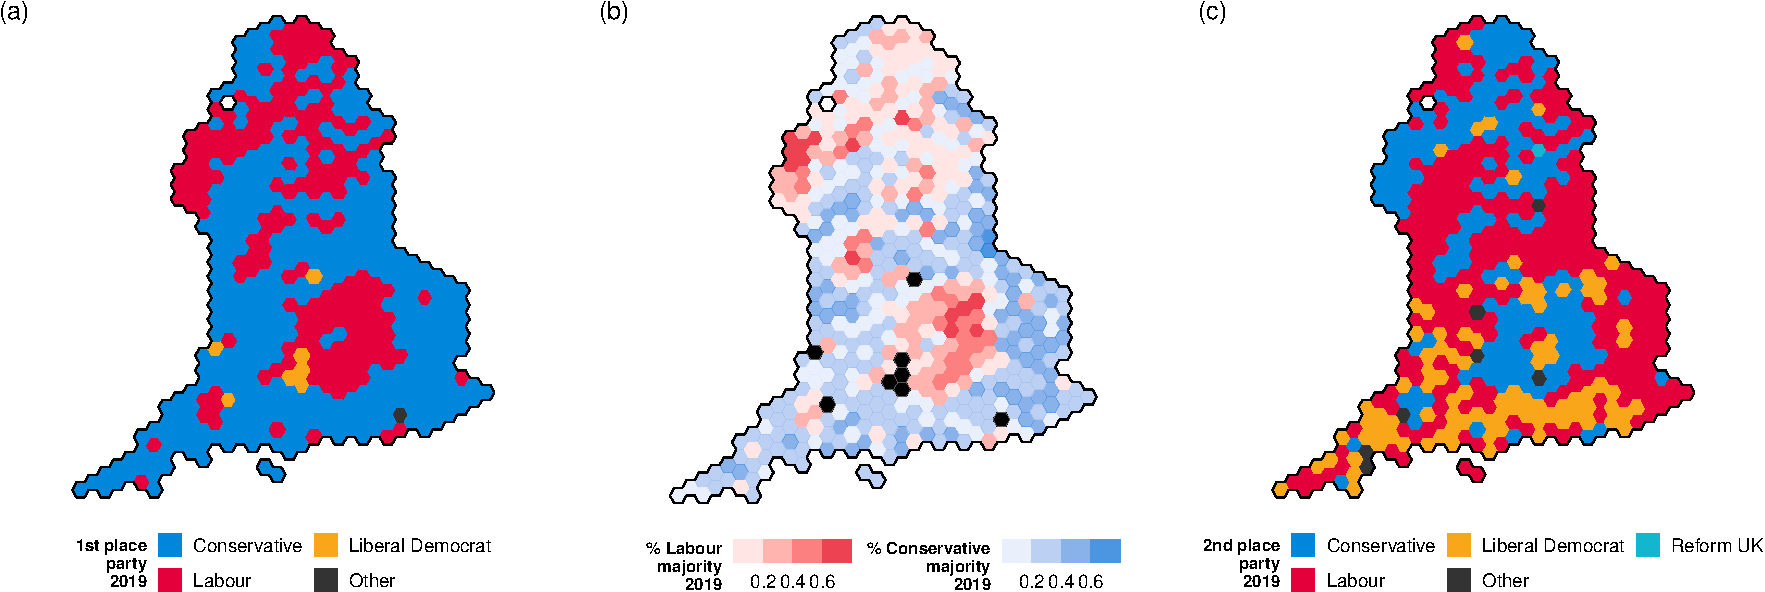
\includegraphics[width=1\linewidth]{jrss_resubmission3_files/figure-latex/figplacement-1} \caption{(a) First place parties by constituency in 2019, (b) majority as a proportion of total votes cast for Conservative and Labour seats, and (c) second place parties by constituency in 2019. All constituencies are reprojected to 2024 boundaries.}\label{fig:figplacement}
\end{figure*}

\subsection{Spatial structures}\label{spatial-structures}

When discussing space in these models, we will be concerned with
vertical location as part of a tree with regions as its branches (Figure
\ref{fig:figregionstree}), and horizontal location as captured by
contiguity (Figure \ref{fig:figspatial}). The nine regions of England
which will form part of the modelling process and future discussion are
mapped in Figure \ref{fig:figregionstree}. They are the highest tier of
sub-national division in England. They have a history of association as
former constituencies for European Parliament elections, between 1994
and 2011 they had partly devolved functions, and they were previously
the first level NUTS regions\footnote{Nomenclature of Territorial Units
  for Statistics (NUTS) is a Eurostat geocode standard for referencing
  the administrative divisions of countries for statistical purposes.}
within the European Union.

When describing connectivity between constituencies in a neighbourhood
matrix, as is required for ICAR models, the presence of islands or
otherwise disconnected units can lead to issues with computation. While
there are no longer any island constituencies in England after the
division of the Isle of Wight into two separate seats, we are still left
with the situation where the constituencies of Isle of Wight East and
West are entirely separate from the rest of the graph. The island is
served by two regular ferry services which facilitate commuting for
work, socialising and cultural exchange in a way that is consistent with
the theory of how voter interaction can lead to neighbourhood effects.
For this reason, using the package \texttt{sfislands}
\citep{sfislands2024}, additional neighbour connections have been added
between Isle of Wight West and New Forest West, and between Isle of
Wight East and Gosport. These correspond to the ferry connection routes.
Even though Reform UK only competed in 521 out of 542 constituencies,
this relative sparsity did not lead to any disconnected units. The
resultant neighbourhood structures for Labour and Reform UK can be seen
in Figures \ref{fig:figspatial} (a) and (b) respectively. The
Conservative and Liberal Democrat contiguity maps, with 541 competing
constituencies, closely resemble that of Labour.

\begin{figure*}[th]

{\centering 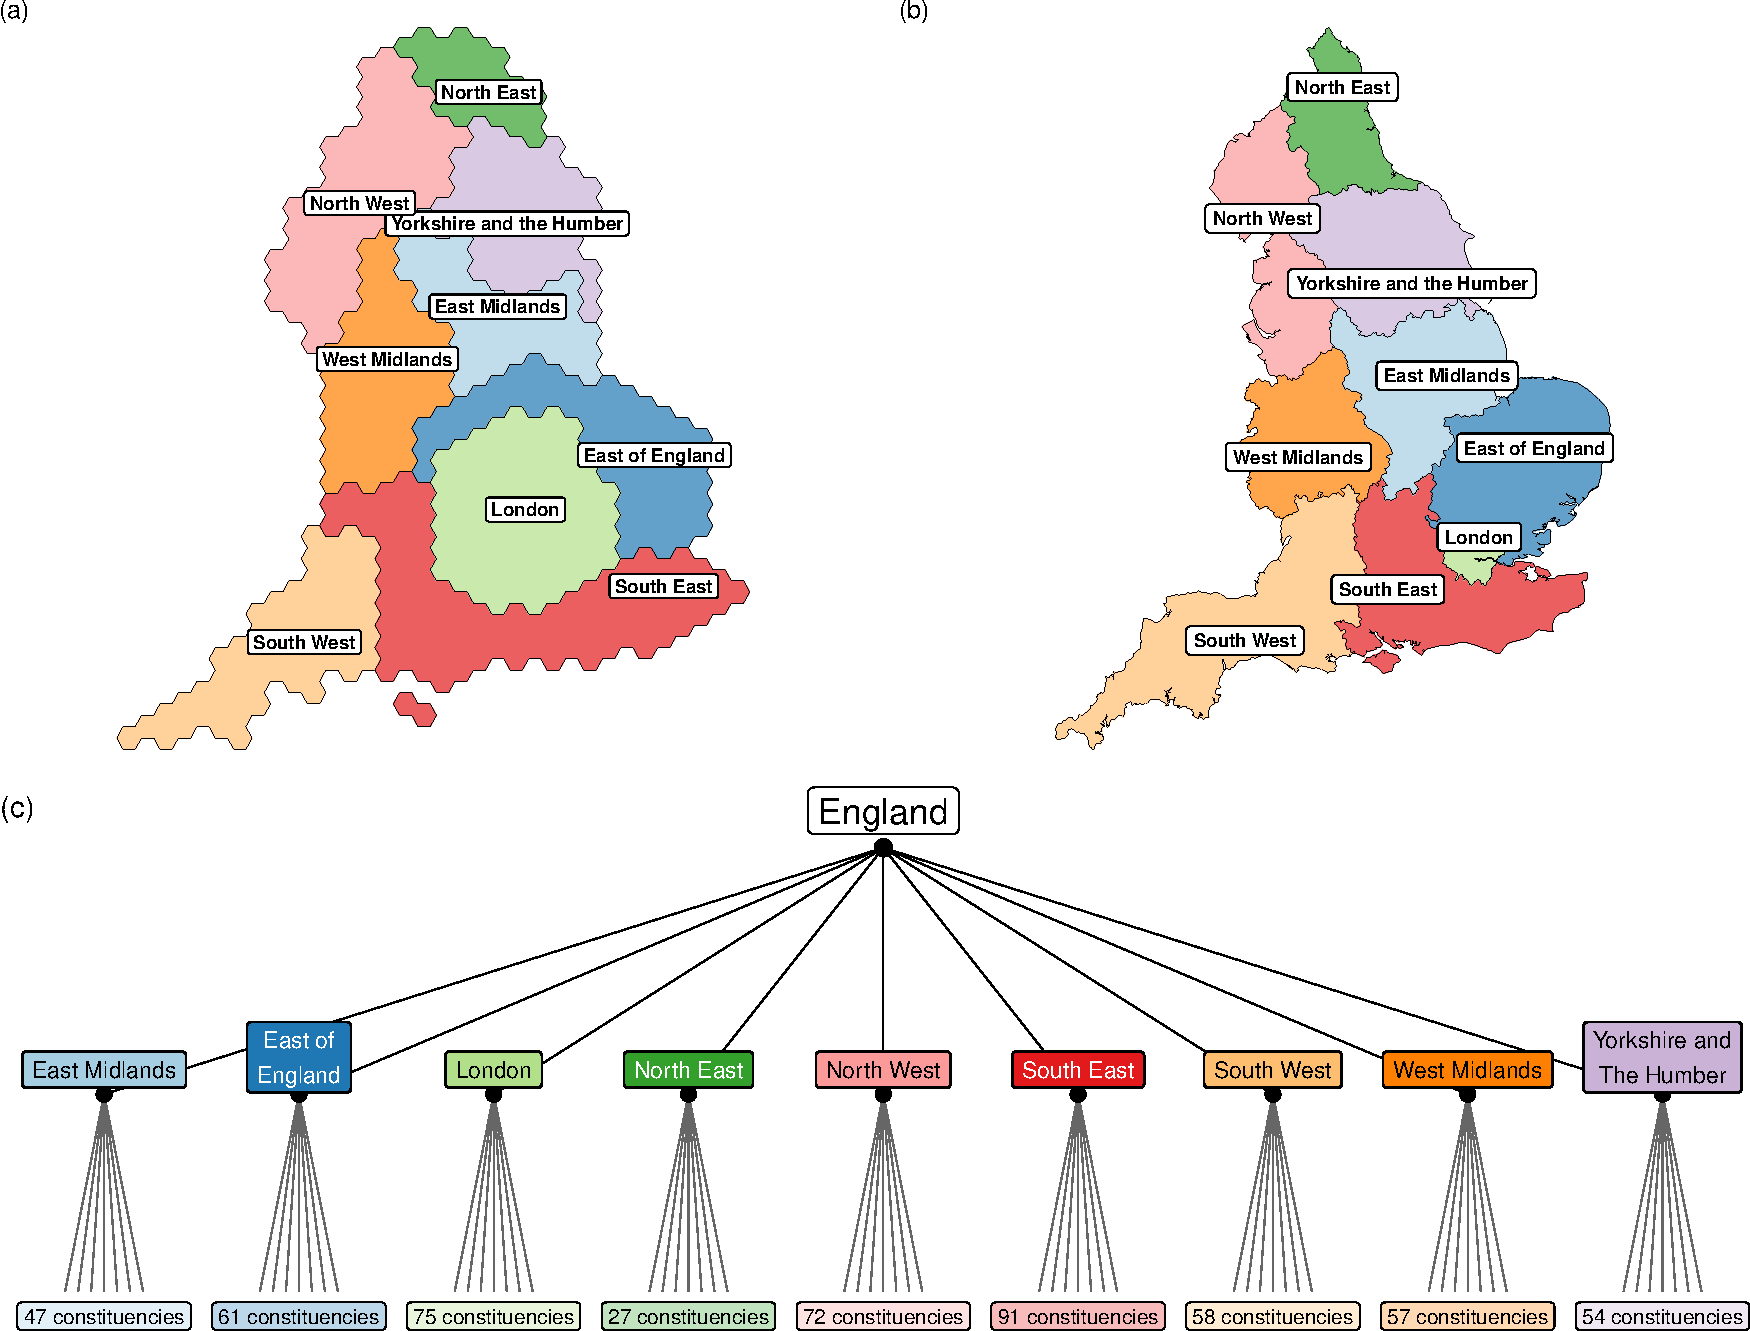
\includegraphics[width=0.9\linewidth]{jrss_resubmission3_files/figure-latex/figregionstree-1} 

}

\caption{Regions of England corresponding to (a) constituency hexagon maps and (b) regular projection. (c) Constituencies and regions of England visualised as a hierarchical tree structure. This can be seen as vertical modelling because only constituencies which branch from a common higher level region are assumed to share share similarities.}\label{fig:figregionstree}
\end{figure*}

\begin{figure*}[th]

{\centering 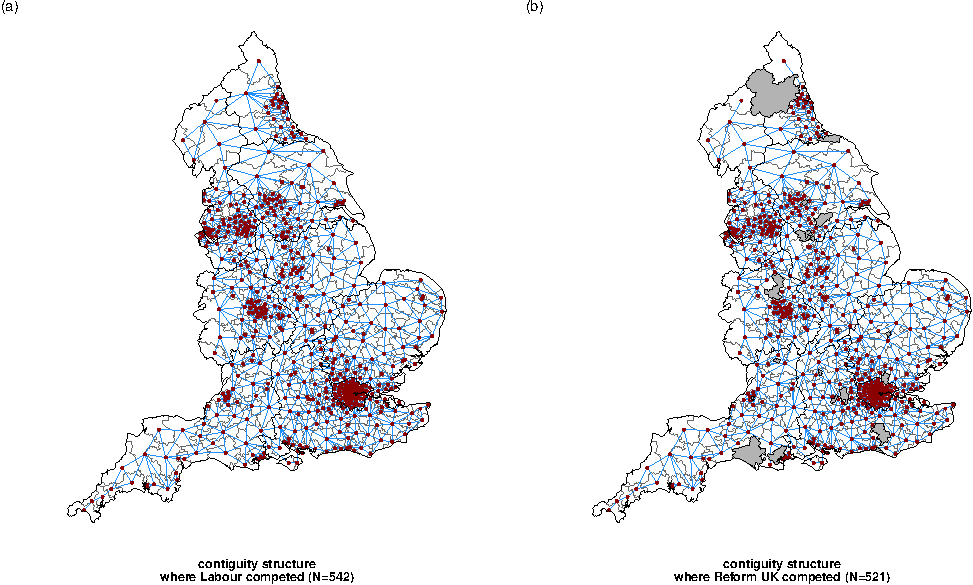
\includegraphics[width=1\linewidth]{jrss_resubmission3_files/figure-latex/figspatial-1} 

}

\caption{Constituencies linked according to queen contiguity for (a) Labour and (b) Reform UK, with an additional connection made between each Isle of Wight constituency and the mainland constituency providing ferry connection. All contiguities are free to cross region boundaries. Conservative and Liberal Democrat contiguity structures (not mapped) only differ from Labour by one constituency each. In (b), constituencies where Reform UK did not compete are shown in grey.}\label{fig:figspatial}
\end{figure*}

\section{Methods}\label{methods}

\subsection{Non-spatial model}\label{non-spatial-model}

Prior to an examination of the relative merits of different spatial
processes, we first seek to establish that there are indeed such
processes which need to be accounted for. The proposed general structure
for this model, without incorporating any spatial information, is a
Poisson generalised linear model where the dependent variable \(Y_i\) is
the count of the number of votes cast for a party in each constituency.
We seek to model this as a linear combination of variables via a log
link function. One such group of variables, as discussed above, is a set
of covariates from the census. These have been used in previous models
of electoral behaviour and serve as proxies for a broad range of
socio-economic conditions. We also control for the political status quo
ante by including as predictors the first and second placed parties from
the previous election, the size of the majority, and its interaction
with the second-placed party. An offset of the log of the total number
of votes cast controls for different exposures due to the varying sizes
of electorates by constituency. The model is fitted in a Bayesian
framework in R using the \texttt{brms} package \citep{brms2017}. To
assess convergence in these and subsequent models, we considered the
convergence diagnostic R-hat \citep{Vehtari2021}, as well as the
individual parameter trace plots.

Such a model structure has the following likelihood for the distribution
of votes cast in each constituency \(i\):

\[
Y_i \sim \text{Poisson}(\mu_i), 
\]

where

\[
\log(\mu_i) = \mathbf{x}_i^\top \boldsymbol{\beta} + \text{offset}_i
\]

The covariates in the \(\mathbf{x}_i^\top \boldsymbol{\beta}\) component
are arranged according to the structure in Table
\ref{tab:tabcovariates}. We assign weakly informative but proper priors,
\(\text{Normal}(0, 10)\), to all \(\beta\) parameters, reflecting
minimal prior knowledge or assumptions about their values.

\begin{table*}

\caption{\label{tab:tabcovariates}Covariates with a brief description, classified as either coming from the 2021 census or the results of the previous election.}
\centering
\fontsize{8}{10}\selectfont
\begin{tabular}[t]{>{\raggedleft\arraybackslash}p{4cm}>{\raggedright\arraybackslash}p{12cm}}
\toprule
Explanatory Variables & Description\\
\midrule
\addlinespace[0.3em]
\hline
\multicolumn{2}{l}{\textbf{census 2021}}\\
\hspace{1em}degree & scaled proportion of constituency population with a degree\\
\hspace{1em}not good health & scaled proportion of constituency population reporting fair, bad, or very bad health\\
\hspace{1em}white & scaled proportion of constituency population of white ethnicity\\
\addlinespace[0.3em]
\hline
\multicolumn{2}{l}{\textbf{status quo ante}}\\
\hspace{1em}first-placed party 2019 & winner from the previous election\\
\hspace{1em}second-placed party 2019 & closest party to winner from previous election\\
\hspace{1em}marginality & scaled difference between winning party and closest rival, as proportion of total votes\\
\hspace{1em}interaction of second-placed party and majority & influence of marginality can vary according to closest competitor\\
\bottomrule
\end{tabular}
\end{table*}

When we fit the model described above, which contains no spatial
components, a visual examination of its Pearson residuals, mapped in
Figure \ref{fig:fignonspatial}, shows clear spatial patterns. We see, at
constituency level, clusters of positive and negative residuals,
suggesting that neighbours have a tendency to be similar to neighbours.
At a regional level, we can see that some regions display similarities
which are quite different to those of others.

\begin{figure*}[th]
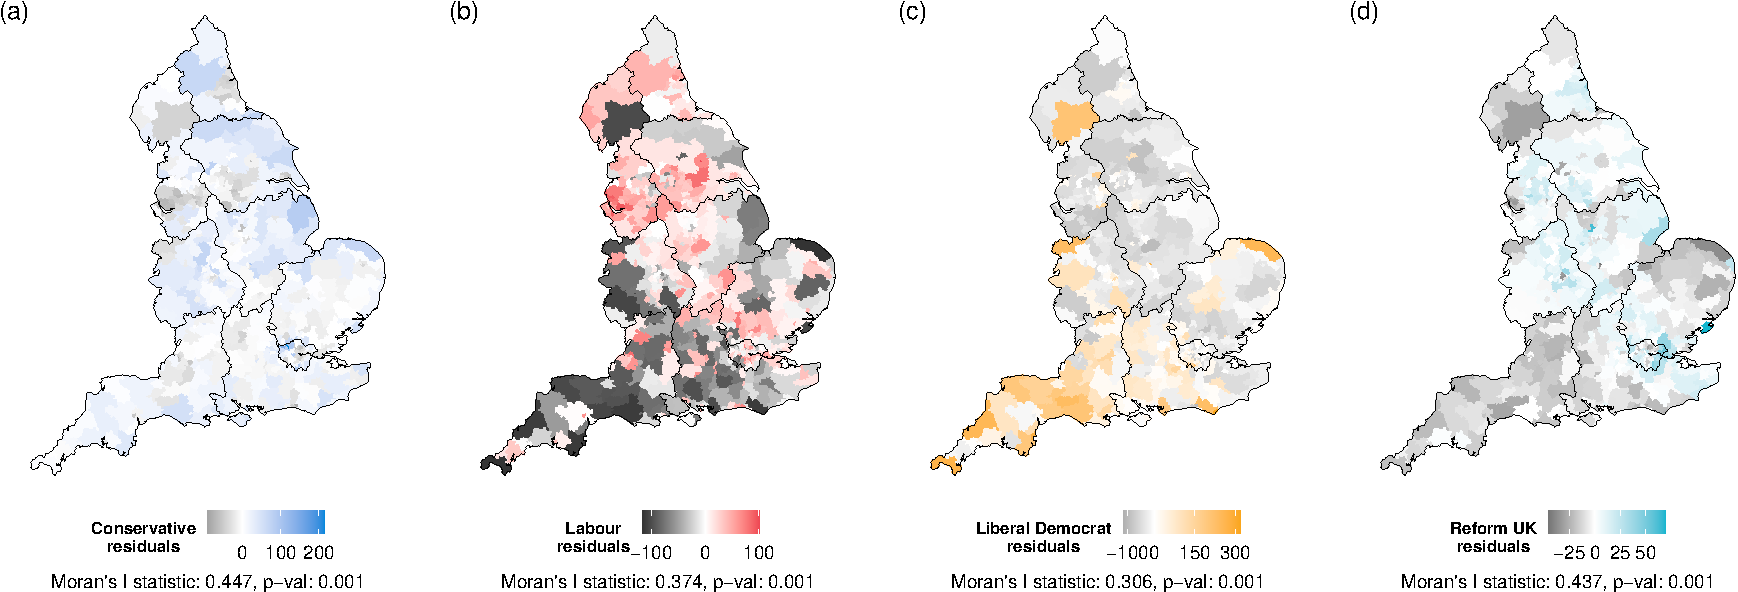
\includegraphics[width=1\linewidth]{jrss_resubmission3_files/figure-latex/fignonspatial-1} \caption{(a-d) Pearson residuals from non-spatial models for each party. Clusters of positive and negative residuals are visible, in addition to regional patterns, suggesting the presence of spatial processes which have not been accounted for. Further evidence for this is provided by a Moran's-I statistic of spatial autocorrelation for each set of residuals, and the p-values of hypothesis tests for random spatial distribution of values.}\label{fig:fignonspatial}
\end{figure*}

\subsection{Spatial models}\label{spatial-models}

The presence of these patterns suggests our model could be improved by
accounting for spatial processes. We allow for the possibility that
these could be at constituency level, region level, or both. With this
in mind, seven further candidate models are fitted for each party
containing different combinations of hypothesised processes, as
summarised in Table \ref{tab:tabmodsummary}.

For Models 1 and 2, we take the non-spatial model described above and
additionally include region random effects only. In the case of Model 1,
each effect is modelled as a dummy variable, considered to come from an
independent sample. For Model 2, these effects are drawn from a common
distribution of region effects as is the case in hierarchical modelling
frameworks.

Model 3 includes only constituency level effects, where we account for
the theory that the behaviour of voters in one constituency is likely to
be similar to that of its neighbours using an ICAR process. This
enforces a constant degree of spatial smoothing across the surface.
Model 4 is the BYM2 variant of the ICAR model with a combination of
spatially structured and unstructured effects at constituency level,
whose relative proportion is also estimated.

Models 5 and 6 combine the region effects of Models 1 and 2 respectively
with the ICAR component of Model 3. These fall into the category of
hierarchical spatial autoregressive modelling (HSAM), as previously
discussed.

Finally, Model 7 contains a novel feature. Despite only featuring a
constituency level ICAR component, in this scenario we account for
regional variation by dropping the constraint that the standard
deviation of the constituency level effects is constant, and allow it to
vary by region. This allows the degree of spatial cohesion to be
modelled and for this to be reflected in the resulting ICAR component.
In some parts of the country, there may be a stronger or weaker tendency
to behave like your neighbours than in other places. This feature allows
a regional effect to operate in a more subtle way than by simply raising
or lowering the mean region level through a random effect.

Models 1-6 are fitted in R using the \texttt{brms} package which relies
on implementations by \citet{Morris2019}. Model 7 uses the
\texttt{rstan} package \citep{rstan2024} with a modification of the Stan
code of Model 3, as generated using the \texttt{brms} function
\texttt{get\_stancode()}.

A summary of the structural component of each model, \(\log(\mu_i)\) or
\(\log(\mu_{ik})\) as appropriate for \(i\) constituencies and \(k\)
regions, and a brief explanation are shown in Table
\ref{tab:tabmodsummary2}.

\begin{table*}

\caption{\label{tab:tabmodsummary}Type of spatial process(es) incorporated in each model, and whether they occur at region level, constituency level, or both.}
\centering
\fontsize{8}{10}\selectfont
\begin{tabular}[t]{cll}
\toprule
Model & Constituency Spatial Effect & Region Spatial Effect\\
\midrule
\addlinespace[0.3em]
\hline
\multicolumn{3}{l}{\textbf{non-spatial}}\\
\hspace{1em}non-spatial & --- & ---\\
\addlinespace[0.3em]
\hline
\multicolumn{3}{l}{\textbf{region only}}\\
\hspace{1em}1 & --- & independent region random effects\\
\hspace{1em}2 & --- & region random effects from common distribution\\
\addlinespace[0.3em]
\hline
\multicolumn{3}{l}{\textbf{constituency only}}\\
\hspace{1em}3 & ICAR process & ---\\
\hspace{1em}4 & BYM2 (ICAR process + unstructured effect) & ---\\
\addlinespace[0.3em]
\hline
\multicolumn{3}{l}{\textbf{region and constituency}}\\
\hspace{1em}5 & ICAR process & independent region random effects\\
\hspace{1em}6 & ICAR process & region random effects from common distribution\\
\hspace{1em}7 & ICAR process & varying icar sd by region\\
\bottomrule
\end{tabular}
\end{table*}

\subsubsection{Priors}\label{priors}

As in the non-spatial model, we assign weakly informative but proper
priors, \(\text{Normal}(0, 10)\), to all \(\beta\) parameters,
reflecting minimal prior knowledge or assumptions about their values. In
addition to the census variables and the previous election effects, such
priors also apply to region effects where they form a part of the model.

The priors for the two different types of ICAR component, \(\phi_i\) and
\(\phi_{ik}\), are defined as follows. When incorporating an ICAR
process, the conditional distribution of a constituency-level spatial
random effect \(\phi_i\), given its neighbours, is:

\[
p(\phi_i \mid \phi_j, {j \neq i}, \sigma) \sim \text{Normal}\left( \frac{\sum_{i \sim j} \phi_i} {d_i}, \frac{\sigma^2}{d_i} \right)
\]

where \(d_i\) is the number of neighbours for constituency \(i\), and
\(i \sim j\) refers to pairs of neighbouring constituencies. The
individual spatial random variable \(\phi_i\) for constituency \(i\)
which has a set of neighbours \(j \neq i\) whose cardinality is \(d_i\),
is Normally distributed with a mean equal to the average of its
neighbours. Its variance decreases as the number of neighbours
increases.

The joint distribution for the vector of all spatial random effects
\(\boldsymbol{\phi} = (\phi_1,...,\phi_N)\) can be written as a pairwise
difference:

\[
p(\boldsymbol{\phi} \mid \sigma) \propto \exp \left( -\frac{1}{2\sigma^2} \sum_{i \sim j} (\phi_i - \phi_j)^2 \right)
\]

This enforces similarity among neighbouring locations. If locations
\(i\) and \(j\) are neighbours, their effects \(\phi_i\) and \(\phi_j\)
are penalised for being different.

To ensure identifiability, a soft sum-to-zero constraint is applied:

\[
\sum_{i=1}^N \phi_i \sim \text{Normal}(0, 0.001 \cdot N)
\]

Instead of this \(\phi_i\) ICAR effect, the BYM2 formulation in Model 4
includes a random effect \(\psi_i\) which is a combination of structured
(ICAR) and unstructured effects at constituency level:

\[
\psi_i = \sigma\sqrt{1-\rho} \, \upsilon_i + \sqrt{\rho} \, \phi_i^*
\]

where \(\sigma\) is the overall standard deviation, \(\phi_i^*\), the
spatially structured effect, is a scaled version of the ICAR prior with
unit variance, \(\upsilon_i\) represents unstructured noise, with
\(\upsilon_i \sim \text{Normal}(0, 1)\), and \(\rho\) is the proportion
of spatial variance in the mixing of these structured and unstructured
components. A proper, uninformative prior of \(\text{Beta}(1,1)\),
uniform in the interval {[}0,1{]}, is used for \(\rho\). A value of 0
for \(\rho\) implies that all spatial variation is unstructured
(independent random effects) while a value of 1 is equivalent to a pure
ICAR model.

In Model 7, where the smoothness of the ICAR effect is allowed to vary
by region \(k\), the spatial prior changes to the following, where
\(\sigma_k\) represents a different standard deviation for each region:

\[
p(\phi_{ik} \mid \phi_j, {j \neq i}, \sigma_{k}) \sim \text{Normal}\left( \frac{\sum_{i \sim j} \phi_{ik}} {d_i}, \frac{\sigma^2_{k}}{d_i} \right)
\]

The soft sum-to-zero constraint, this time for \(\phi_{ik}\), remains
unchanged. The hyper-parameters \(\sigma\) or \(\sigma_k\), representing
the fixed or varying smoothness of the ICAR component respectively were
initially assigned uniform priors. This, however, led to very
inefficient sampling. Instead, a tighter prior was chosen with a
probability distribution function derived from a generator of random
values from a Student-t distribution with mean 0, standard deviation
2.5, and degrees of freedom 3, where the absolute value of each draw is
used, implying an expectation that the value will be close to zero but
not ruling out the possibility of much larger values:

\[
\sigma \sim \text{Student-t}(3, 0, 2.5), \quad \sigma > 0
\]

This achieved similar results to the uniform prior but with much less
computation time. This prior is also used for the \(\sigma_R\)
hyper-parameter of the \(\gamma_k\) region effect distribution in Models
2 and 5.

\begin{table*}

\caption{\label{tab:tabmodsummary2}Structure of each model, showing which spatial processes are included.}
\centering
\fontsize{8}{10}\selectfont
\begin{tabular}[t]{cl>{\raggedright\arraybackslash}p{6.5cm}}
\toprule
Model & Description & Note\\
\midrule
\addlinespace[0.3em]
\hline
\multicolumn{3}{l}{\textbf{non-spatial}}\\
\hspace{1em}non-spatial & $ \log(\mu_i) = \mathbf{x}_i^\top \boldsymbol{\beta} + \text{offset}_i $ & where $\mathbf{x}_i^\top \boldsymbol{\beta}$ contains explanatory variables from census and previous election\\
\addlinespace[0.3em]
\hline
\multicolumn{3}{l}{\textbf{region only}}\\
\hspace{1em}1 & $ \log(\mu_i) = \tilde{\mathbf{x}}_i^\top\tilde{\boldsymbol{\beta}} + \text{offset}_i $ & where $\tilde{\mathbf{x}}_i^\top\tilde{\boldsymbol{\beta}}$ includes an additional region component\\
\hspace{1em}2 & $ \log(\mu_{ik}) = \mathbf{x}_i^\top \boldsymbol{\beta} + \gamma_k + \text{offset}_i $ & where $\gamma_k$ is a region random effect from a common distribution, with $\gamma_k \sim \text{Normal}(0, \sigma^2_R)$\\
\addlinespace[0.3em]
\hline
\multicolumn{3}{l}{\textbf{constituency only}}\\
\hspace{1em}3 & $ \log(\mu_i) = \mathbf{x}_i^\top \boldsymbol{\beta} + \phi_i + \text{offset}_i $ & where $\phi_i$ is a constituency random effect from an ICAR process\\
\hspace{1em}4 & $ \log(\mu_i) = \mathbf{x}_i^\top \boldsymbol{\beta} + \psi_i + \text{offset}_i $ & where $\psi_i$ is a mixture of spatial effects and unstructured noise according to a mixing parameter $\rho$\\
\addlinespace[0.3em]
\hline
\multicolumn{3}{l}{\textbf{region and constituency}}\\
\hspace{1em}5 & $ \log(\mu_i) = \tilde{\mathbf{x}}_i^\top\tilde{\boldsymbol{\beta}} + \phi_i + \text{offset}_i $ & region effects of model 1 and constituency effects of model 3\\
\hspace{1em}6 & $ \log(\mu_{ik}) = \mathbf{x}_i^\top \boldsymbol{\beta} + \gamma_k + \phi_i + \text{offset}_i $ & region effects of model 2 and constituency effects of model 3\\
\hspace{1em}7 & $ \log(\mu_{ik}) = \mathbf{x}_i^\top \boldsymbol{\beta} + \gamma_k + \phi_{ik} + \text{offset}_i $ & where $\phi_{ik}$ allows for varying standard deviation by region in the ICAR process\\
\bottomrule
\end{tabular}
\end{table*}

\section{Exploratory simulations}\label{exploratory-simulations}

Before fitting a sequence of competing models for each party, we first
seek to verify that the proposed approach of using marginal likelihoods
to determine relative plausibility is effective. If the underlying
spatial structure is known, will the corresponding model emerge as the
most plausible? This is done using some exploratory simulations.

To create a realistic but less computationally intensive geographical
setting, we extract the 101 constituencies from the regions of Yorkshire
and the Humber and the East of England. We then divide these into six
pseudo-regions, with each containing only contiguous constituencies, by
a process of hierarchical clustering about their centroid positions (see
Figure \ref{fig:pseudoregions}).

\begin{figure*}[th]

{\centering 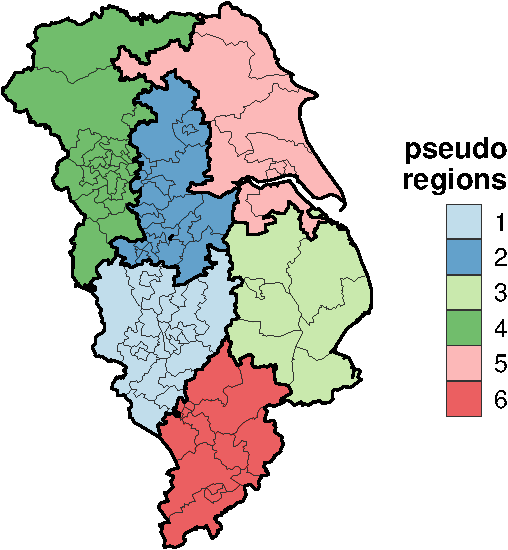
\includegraphics[width=0.25\linewidth]{jrss_resubmission3_files/figure-latex/pseudoregions-1} 

}

\caption{A spatial structure for performing simulations is created by extracting the boundaries of constituencies from the East of England and Yorkshire and The Humber and dividing them into 6 pseudo-regions, each containing only contiguous constituencies, by a process of hierarchical clustering about their centroid positions.}\label{fig:pseudoregions}
\end{figure*}

Three distinct types of spatially structured data are randomly
generated, each with five independent replicates: the first type follows
an ICAR structure (as in Model 3); the second combines an ICAR structure
with a region effect (Model 5); and the third uses an ICAR structure
with region-specific variance \(\sigma_k\) (Model 7).

We then fit our eight competing models to each of the simulated
structures and estimate the log marginal likelihood using the
\texttt{bridgesampling} package \citep{Gronau2017}, which provides a
stable and accurate estimate via bridge sampling
\citep{meng1996simulating}. For Models 3 and 5, we begin with a
relatively tight ICAR variance (\(\sigma\)) of 0.7. In the Model 5
structure, a range of six region effects is introduced: --1.5, 1, --0.5,
0.5, 1, and 1.2. For Model 7, samples are generated using six
region-specific ICAR variances (\(\sigma_k\)): 0.2, 0.6, 1, 1.4, 1.8,
and 2.2. Figure \ref{fig:narrowsds} displays each of these structures,
with the three most plausible models (based on log marginal likelihood)
shown below each map. In all cases, the correct model is preferred.

Additional noise is then introduced by increasing the ICAR \(\sigma\)
value to 1.3 in Models 3 and 5 (see Figure \ref{fig:widesds}). In one of
the five replicates, the model with region-specific ICAR variance
(\(\sigma_k\)) was marginally preferred over the true underlying ICAR
structure. This outcome is expected: when spatial data are generated
with high noise, it is not surprising that a more flexible structure
(such as varying \(\sigma_k\)) may occasionally offer a better or
equally good fit. In all other cases, the correct models were preferred.

While this exploratory simulation is not exhaustive, it provides
preliminary evidence that the method can correctly identify the true
underlying structure as the most plausible among competing alternatives,
rather than favouring, for example, the model with the greatest
complexity.

\begin{figure*}[th]

{\centering 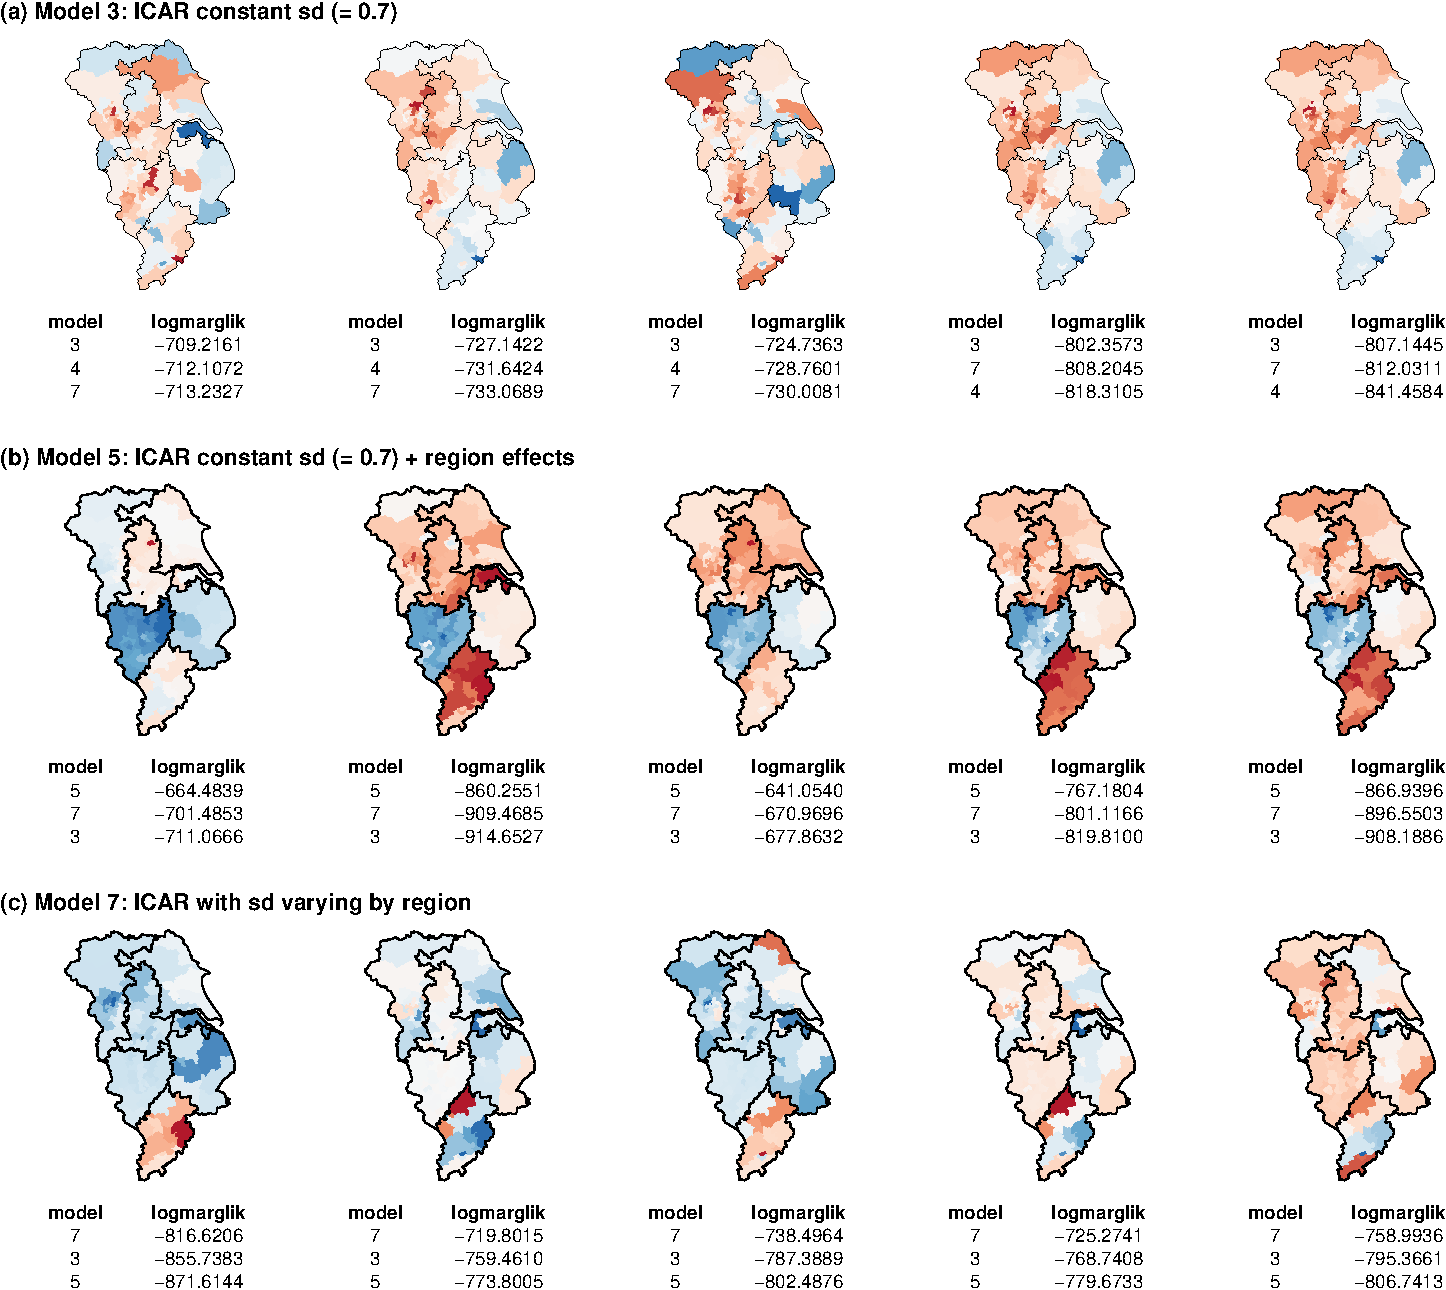
\includegraphics[width=0.9\linewidth]{jrss_resubmission3_files/figure-latex/narrowsds-1} 

}

\caption{Each row consists of five random samples of data with a known spatial association. The first row are ICAR, the second are ICAR with an additional region effect, the third are ICAR with standard deviation varying by region. In all cases, the use of marginal likelihoods identifies the correct underlying spatial structure as the most plausible.}\label{fig:narrowsds}
\end{figure*}

\begin{figure*}[th]

{\centering 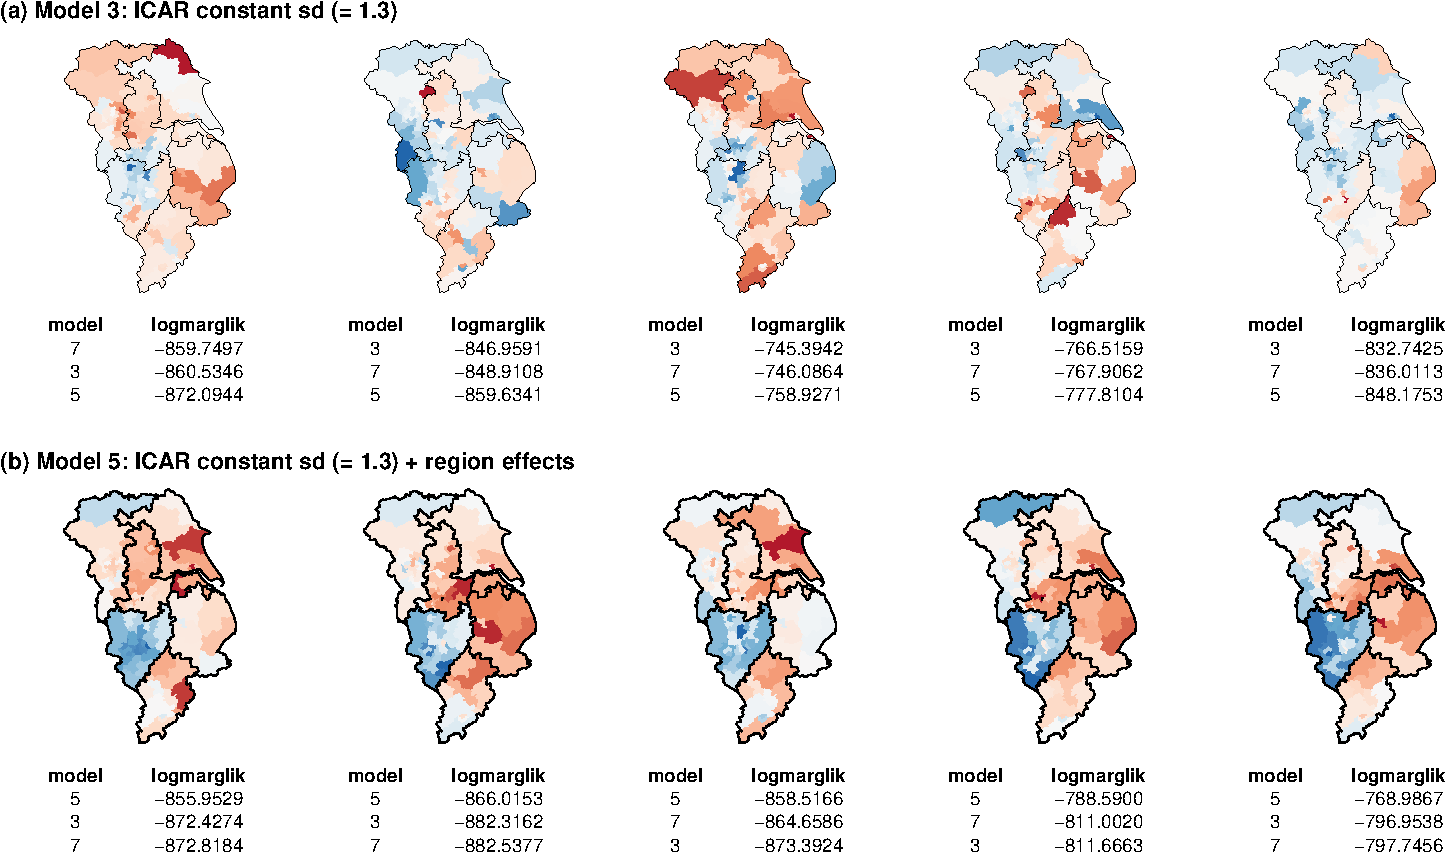
\includegraphics[width=0.9\linewidth]{jrss_resubmission3_files/figure-latex/widesds-1} 

}

\caption{Each row consists of five random samples of data with a known spatial association. The first row are ICAR, the second are ICAR with an additional region effect. These samples have a larger standard deviation of 1.3 meaning there is less spatial cohesion than in the previous example. In almost all cases, the use of marginal likelihoods identifies the correct underlying spatial structure as the most plausible.}\label{fig:widesds}
\end{figure*}

\section{Results}\label{results}

\subsection{Model comparison}\label{model-comparison}

For each party, we evaluate eight competing models, each representing a
different probabilistic structure that could have generated the observed
voting data. We compute the log marginal likelihood of each model using
bridge sampling. These marginal likelihoods can also be expressed as
Bayes factors, enabling evidence-based comparison between models.

A Bayes factor compares the likelihood of the observed data under two
competing models. Specifically, the Bayes factor for Model 1 relative to
Model 2 quantifies how much more likely the data are under Model 1 than
under Model 2. Values greater than 1 indicate evidence in favour of
Model 1, while values less than 1 support Model 2. The magnitude of the
Bayes factor reflects the strength of this evidence. We interpret these
values using the scale proposed by \citet{Lee2014} (an update to the
original guidelines of \citet{jeffreys1939}) as shown in Table
\ref{tab:tablewagenmakers}.

\begin{table*}

\caption{\label{tab:tablewagenmakers}Lee and Wagenmakers' interpretation of Bayes factors, quantifying how much more likely data are under one model compared to another.}
\centering
\fontsize{8}{10}\selectfont
\begin{tabular}[t]{l|l}
\hline
Bayes Factor Range & Evidence Supporting One Model Over Another\\
\hline
$> 0, < 1$ & negative\\
\hline
$\geq 1, < 3$ & anecdotal\\
\hline
$\geq 3, < 10$ & moderate\\
\hline
$\geq 10, < 30$ & strong\\
\hline
$\geq 30, < 100$ & very strong\\
\hline
$\geq 100$ & extreme\\
\hline
\end{tabular}
\end{table*}

Table \ref{tab:tablik} shows the results of comparing the merits of the
eight potential models for each of the four parties using this
classification structure. The models are ranked for each party according
to decreasing log marginal likelihood. Bayes factors are shown comparing
each model to the model immediately below it. Because they have been
ranked, Bayes factor values of less than 1 do not occur. For all sets of
models in Table \ref{tab:tablik}, the most plausible is Model 7, with an
ICAR component whose standard deviation is allowed to vary by region.
The evidence in favour of this model over its closest competitor is in
each case classified as \textit{extreme}. With some minor exceptions,
the order of preference of models is consistent across parties.

\begin{table*}

\caption{\label{tab:tablik}Comparison of models across parties, ranked by decreasing log marginal likelihood, alongside the degree of evidence for model improvement provided by Bayes factor comparison with the model immediately below it. The sequence is generally the same for each party with Model 7 being the most plausible.}
\centering
\fontsize{8}{10}\selectfont
\begin{tabular}[t]{>{\centering\arraybackslash}p{2.1cm}>{\raggedright\arraybackslash}p{2.5cm}>{\raggedright\arraybackslash}p{4cm}>{\raggedleft\arraybackslash}p{2.5cm}>{\raggedright\arraybackslash}p{1.4cm}>{\raggedright\arraybackslash}p{1.4cm}l}
\toprule
Model & Constituency Level Effects & Region Level Effects & Log Marginal Likelihood & Log Bayes Factor & Bayes Factor & Evidence\\
\midrule
\addlinespace[0.3em]
\hline
\multicolumn{7}{l}{\textbf{Conservative}}\\
\hspace{1em}7 & ICAR & varying ICAR sd & -4809.537 & 49 & $>$1e+6 & extreme\\
\hspace{1em}3 & ICAR & --- & -4859.002 & 35 & $>$1e+6 & extreme\\
\hspace{1em}5 & ICAR & independent distributions & -4894.030 & 14 & $>$1e+6 & extreme\\
\hspace{1em}6 & ICAR & common distribution & -4907.638 & 42 & $>$1e+6 & extreme\\
\hspace{1em}4 & BYM2 & --- & -4949.994 & 78000 & $>$1e+6 & extreme\\
\hspace{1em}2 & --- & common distribution & -83402.581 & 35 & $>$1e+6 & extreme\\
\hspace{1em}1 & --- & independent distributions & -83437.307 & 250000 & $>$1e+6 & extreme\\
\hspace{1em}non-spatial & --- & --- & -328526.802 & --- & --- & ---\\
\addlinespace[0.3em]
\hline
\multicolumn{7}{l}{\textbf{Labour}}\\
\hspace{1em}7 & ICAR & varying ICAR sd & -5171.735 & 82 & $>$1e+6 & extreme\\
\hspace{1em}3 & ICAR & --- & -5253.968 & 32 & $>$1e+6 & extreme\\
\hspace{1em}5 & ICAR & independent distributions & -5286.028 & 200 & $>$1e+6 & extreme\\
\hspace{1em}6 & ICAR & common distribution & -5488.055 & 30 & $>$1e+6 & extreme\\
\hspace{1em}4 & BYM2 & --- & -5518.061 & 170000 & $>$1e+6 & extreme\\
\hspace{1em}2 & --- & common distribution & -178712.220 & 30 & $>$1e+6 & extreme\\
\hspace{1em}1 & --- & independent distributions & -178742.703 & 480000 & $>$1e+6 & extreme\\
\hspace{1em}non-spatial & --- & --- & -659934.748 & --- & --- & ---\\
\addlinespace[0.3em]
\hline
\multicolumn{7}{l}{\textbf{Reform UK}}\\
\hspace{1em}7 & ICAR & varying ICAR sd & -4253.464 & 53 & $>$1e+6 & extreme\\
\hspace{1em}3 & ICAR & --- & -4306.382 & 15 & $>$1e+6 & extreme\\
\hspace{1em}4 & BYM2 & --- & -4321.256 & 16 & $>$1e+6 & extreme\\
\hspace{1em}6 & ICAR & common distribution & -4337.488 & 4.7 & 110 & extreme\\
\hspace{1em}5 & ICAR & independent distributions & -4342.195 & 38000 & $>$1e+6 & extreme\\
\hspace{1em}2 & --- & common distribution & -42360.147 & 29 & $>$1e+6 & extreme\\
\hspace{1em}1 & --- & independent distributions & -42389.058 & 27000 & $>$1e+6 & extreme\\
\hspace{1em}non-spatial & --- & --- & -69501.304 & --- & --- & ---\\
\addlinespace[0.3em]
\hline
\multicolumn{7}{l}{\textbf{Liberal Democrat}}\\
\hspace{1em}7 & ICAR & varying ICAR sd & -4713.785 & 25 & $>$1e+6 & extreme\\
\hspace{1em}3 & ICAR & --- & -4739.024 & 22 & $>$1e+6 & extreme\\
\hspace{1em}5 & ICAR & independent distributions & -4760.673 & 230 & $>$1e+6 & extreme\\
\hspace{1em}6 & ICAR & common distribution & -4991.153 & 84 & $>$1e+6 & extreme\\
\hspace{1em}4 & BYM2 & --- & -5074.869 & 250000 & $>$1e+6 & extreme\\
\hspace{1em}2 & --- & common distribution & -258553.477 & 24 & $>$1e+6 & extreme\\
\hspace{1em}1 & --- & independent distributions & -258577.449 & 6e+05 & $>$1e+6 & extreme\\
\hspace{1em}non-spatial & --- & --- & -859667.026 & --- & --- & ---\\
\bottomrule
\end{tabular}
\end{table*}

\subsection{Covariate estimates from optimal
models}\label{covariate-estimates-from-optimal-models}

Having established which of our competing models is most appropriate for
each of the parties, we can examine the posterior distributions of some
parameters from the most favoured models for each party. All of these
distributions are from Model 7. Looking at the socio-economic components
(Figure \ref{fig:figsocecposts}), we can see differences in directions
of association for each party. The proportion of people with a
\emph{degree} is negatively associated with Reform votes, while the
association is positive for the Conservatives and Liberal Democrats. The
opposite is the case for \emph{health not good}, having a suggestion of
positive association with Reform votes and negative for Conservatives
and Liberal Democrats. The proportion of a constituency of \emph{white}
ethnicity is most strongly positively associated with Reform votes, but
is also positive for Labour.

\begin{figure*}[th]

{\centering 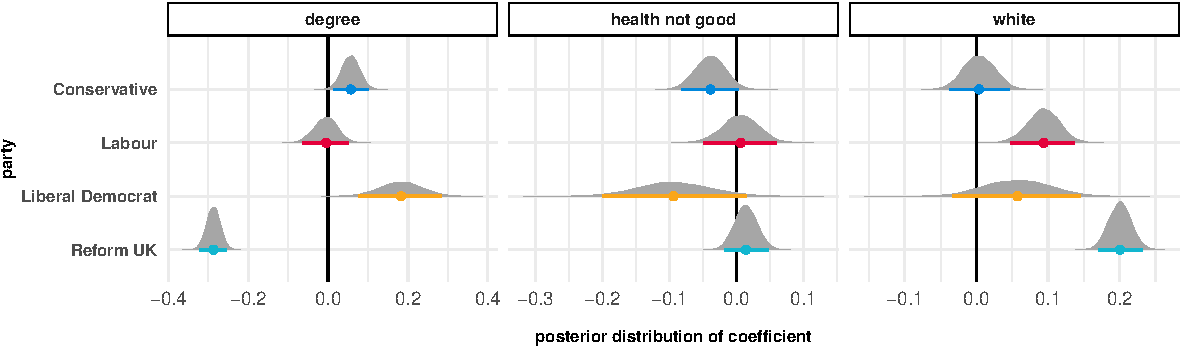
\includegraphics[width=0.85\linewidth]{jrss_resubmission3_files/figure-latex/figsocecposts-1} 

}

\caption{Posterior distributions of coefficients for socio-economic variables from Model 7 for Conservatives, Labour, Liberal Democrats and Reform.}\label{fig:figsocecposts}
\end{figure*}

The associations of votes in 2024 with the winning party from 2019, and
also with the second placed party, the majority, and their interaction
are treated in this example as nuisance variables for control purposes.
Interpretation of their posterior distributions is complicated because
of their calibration with different relative baselines. For this reason,
they are not examined here.

\subsection{Spatial estimates from optimal
models}\label{spatial-estimates-from-optimal-models}

Moving to the spatial components, the mean posterior values of the ICAR
component (which have regionally varying \(\sigma_k\)) are shown as maps
(a-d) in row 1 of Figure \ref{fig:figspatialposts}. Differences in the
degree of smoothness are clearly visible such as in the South West
region for Labour, where strongly negative and positive values occur
contiguously.

The second row (e-h) shows the mean posterior of the varying standard
deviations mapped by region. These varying levels of spatial cohesion
have been split into quintiles. These are quintiles of mean values of
all parties in all regions. At the lower end of the scale, we have
quintiles 1 and 2 in blue, which are `most' and `somewhat' cohesive
respectively. Areas close to median spatial cohesion (`moderate') are
shown in white, with more extreme values (`less' or `least' cohesive)
shown in orange.

Much of the Conservative vote pattern lies within the `moderate'
cohesion category. Exceptions to this are across southern regions where
it is more cohesive and in Yorkshire and the Humber where neighbouring
constituencies are not similar to the neighbours in terms of voting
Conservative. Labour only shows `moderate' levels of cohesion in London.
Its cohesion pattern is split largely along a north-south divide with
neighbouring constituencies showing similar behaviour in the north as
opposed to the south.

The mean posterior ICAR \(\sigma_k\) values for the Liberal Democrats
are all in the higher categories. Those of Reform UK, on the other hand,
are all below the median level (with the exception of London), with most
in fact falling into the category of `most' cohesive. This is consistent
with the notion of that party having a relatively consistent widespread
level of support, although not quite to the extent where the
first-past-the-post system would benefit them.

Plots (i)-(l) on row 3 focus on the 95\% credible intervals rather than
the means of the posterior \(\sigma_k\) values, and place their ranges
within the context of the overall quintile levels. These plots tell a
similar story, showing not only higher values of \(\sigma_k\) for
Liberal Democrat voters, but a greater degree of uncertainty as to their
value.

The results of this model comparison, which show strong evidence of
differences in the level of spatial cohesion of voting patterns for
different parties, clearly raises the question of why this would be the
case. We could hypothesise that it is connected to unaccounted-for
strategic voting, regional organisation, identity, urban versus rural
constituencies, or other factors. There is, however, no evidence for any
of this in the data. Further research would be required to rigorously
investigate this.

\begin{figure*}[th]
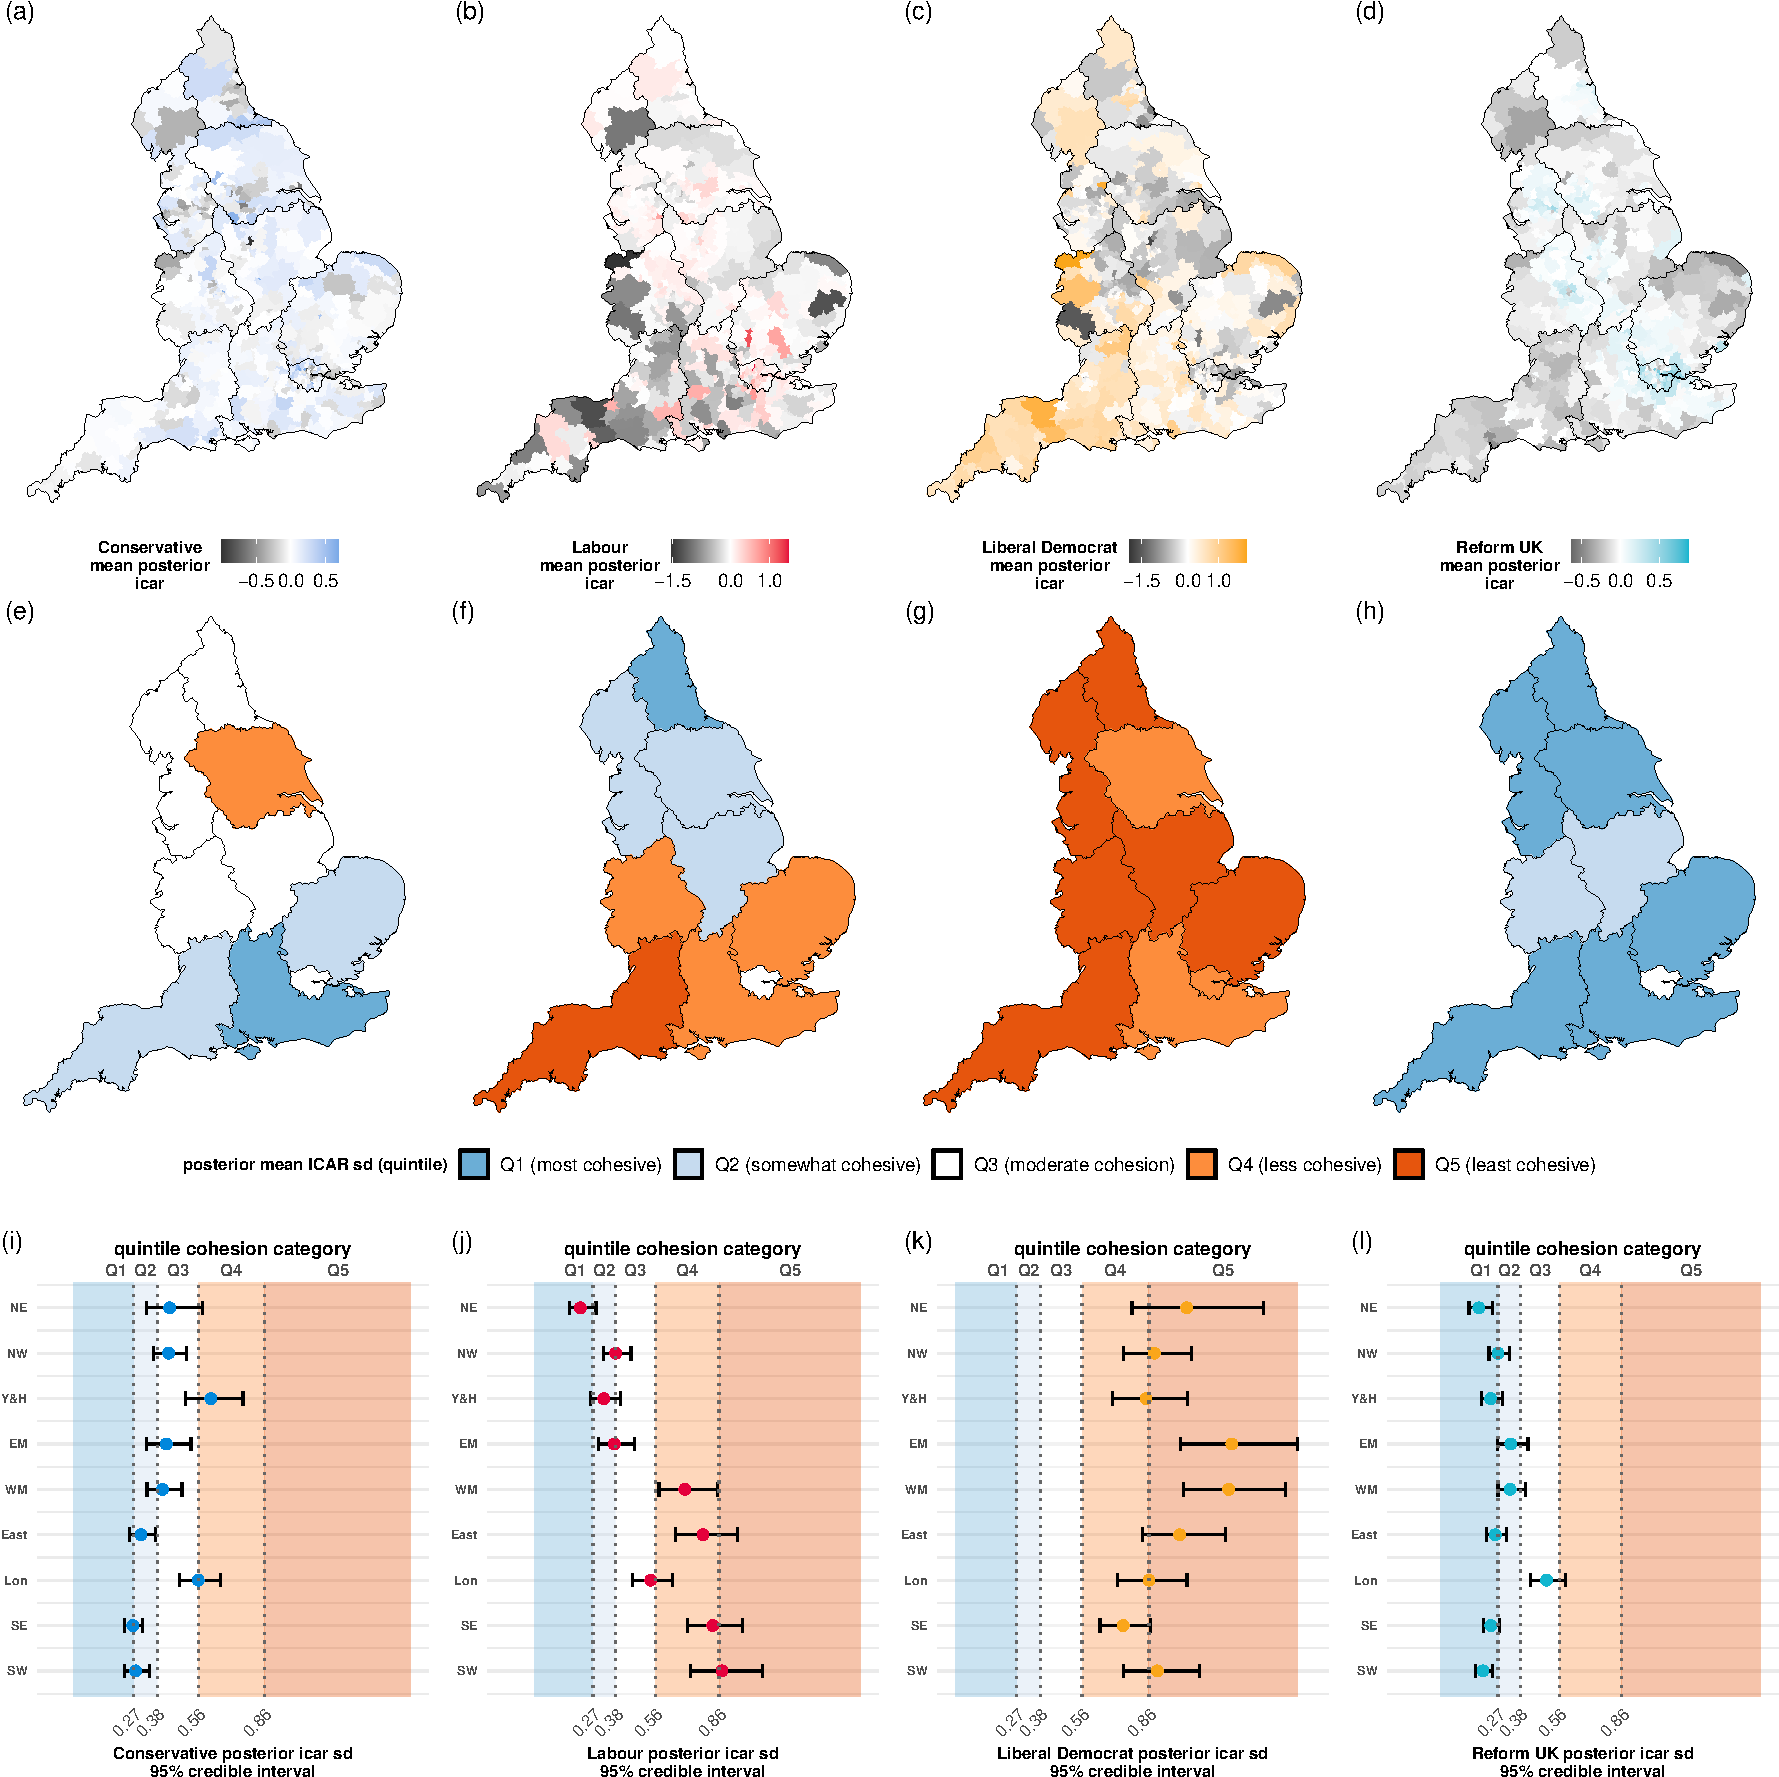
\includegraphics[width=1\linewidth]{jrss_resubmission3_files/figure-latex/figspatialposts-1} \caption{(a-d) Mean posterior of ICAR component of Model 7 for Conservatives, Labour, Liberal Democrats and Reform UK respectively, (e-h) mean posterior value of standard deviation component from Model 7 for each party, varying by region, and (i-l) 95\% credible intervals of the posterior distributions of these varying standard deviations.}\label{fig:figspatialposts}
\end{figure*}

\subsection{Exceedance probabilities}\label{exceedance-probabilities}

Rather than comparing posterior means of spatial cohesion across all
parties using a global average variance, we can instead calculate
exceedance probabilities \citep{Richardson2004} separately for each
party. These represent the posterior probability that a region's
variance \(\sigma_k\) exceeds the party-specific mean, indicating lower
spatial cohesion relative to that party's typical pattern across
England. This within-party approach allows us to identify regions with
unusually weak spatial structure for each party in its own context. The
resulting maps are shown in Figure \ref{fig:figexceedances}.

They show patterns broadly similar to those in Figure
\ref{fig:figspatialposts} for Conservative, Labour and Reform UK voters.
In the case of Liberal Democrat voters, they highlight both the East and
West Midlands as regions with particularly uncohesive voting patterns,
even relative to the already high \(\sigma_k\) values typical of Liberal
Democrat support.

\begin{figure*}[th]
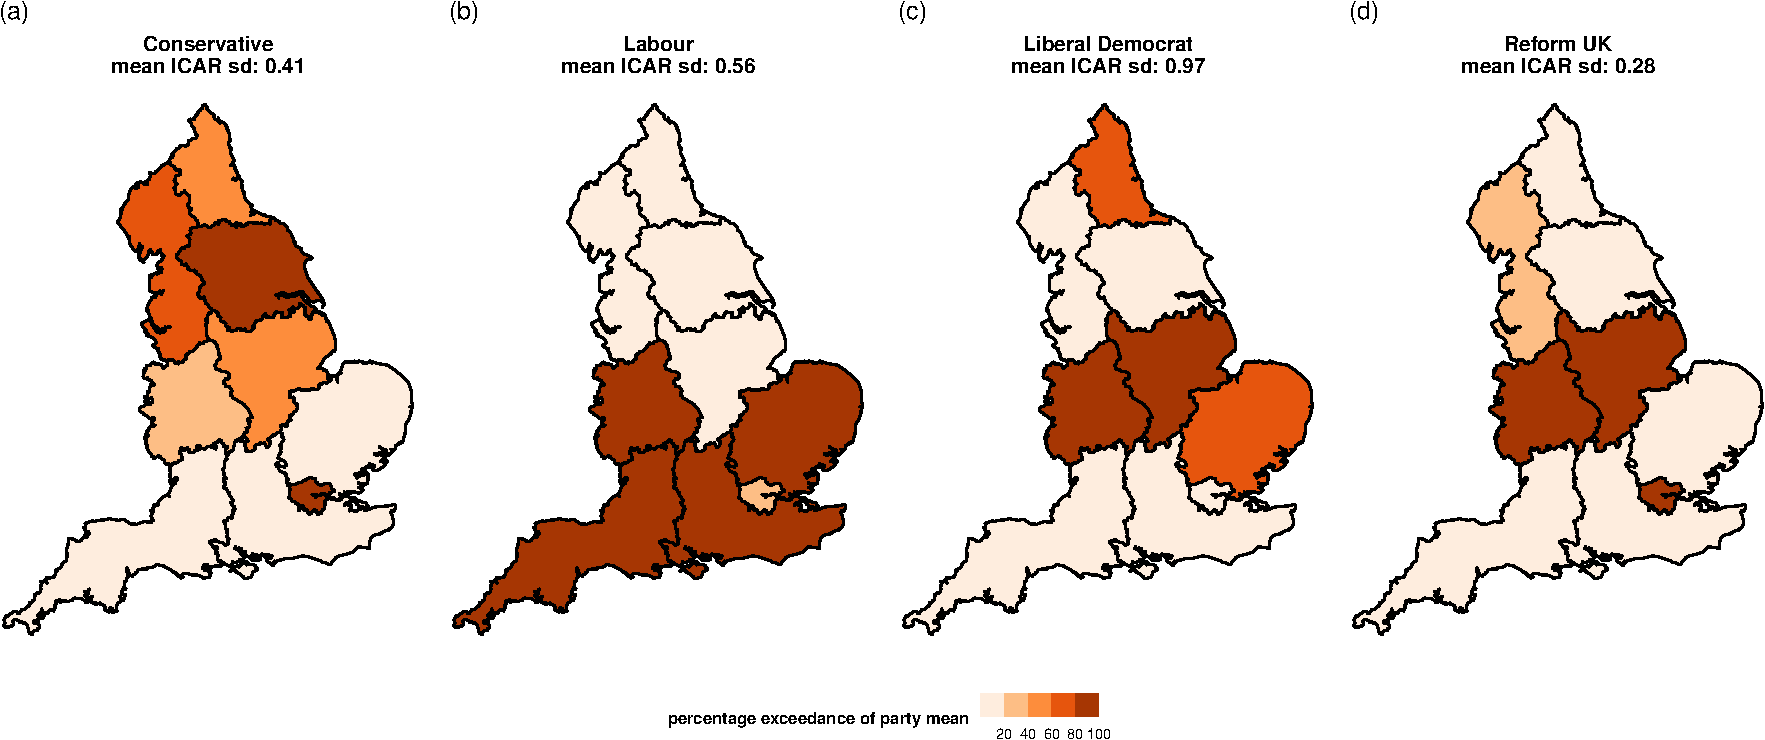
\includegraphics[width=1\linewidth]{jrss_resubmission3_files/figure-latex/figexceedances-1} \caption{Posterior exceedance by region, showing as percentages the posterior probability that a region’s ICAR variance exceeds the party-specific mean (shown above map), indicating lower spatial cohesion relative to that party’s typical pattern across England.}\label{fig:figexceedances}
\end{figure*}

\section{Conclusions}\label{conclusions}

In this paper, we proposed a novel structure for describing spatial
processes occurring simultaneously at different levels. Rather than
combining hierarchical models with a spatially autocorrelated process at
the lowest level, we instead allowed the higher level differences to be
reflected within the ICAR component itself, reflecting varying spatial
cohesion. We constructed these models using a Bayesian framework and
demonstrated how we could judge if our novel structure was more
appropriate than others using log marginal likelihoods and Bayes
factors.

This technique was applied to voting data from the UK, based on a theory
that the tendency for voters in one constituency to behave similarly to
their neighbours might not be the same in all parts of England. Some
regions might demonstrate greater spatial cohesion in terms of electoral
preferences than others. We found evidence that such differences did
exist and that this new model was an improvement over standard ICAR
models for all four of the largest parties. We found that, at a national
scale, votes for Reform UK showed the highest degree of spatial cohesion
between neighbouring constituencies while those for the Liberal
Democrats showed the lowest. On a region by region basis, Conservative
votes were more spatially cohesive in the south relative to the north,
while the opposite was the case for Labour.

ICAR models with or without an additional hierarchical component are
common in many areas of spatial analysis. This concept of allowing
spatial cohesion to vary by region has wider application potential than
just to voting data. In epidemiological modelling, for example, it might
be desirable to allow the intensity of the spread of disease to be
similarly variable by region. Rather than using region random effects,
perhaps the process could be better captured by focussing only on the
spatially smoothed ICAR component but allowing its degree of smoothness
to vary. This idea could also be applied to studies of crime, social
inequality, public health, environmental issues, ecology and housing
markets. Within each of these areas, the meaning of the varying standard
deviation of the ICAR structure would have its own interpretation.

It is this area of interpretation which may be one of the main
limitations of this model. A combination of hierarchical effects and a
spatially smooth process lends itself to a more standard and less
complicated narrative than discussion of spatial cohesion. However, the
explicit measure of spatial cohesion which this model provides may be of
interest to test specific theories. Also, if the more complex model is
deemed more plausible, this can raise questions about the simpler
model's assumptions.

Another limitation which should be mentioned is the additional
computational burden introduced by the varying \(\sigma_k\) parameter.
For this reason, we only sought to compare one instance of its use (in
the form of Model 7) with a number of other candidate models, but there
is scope for incorporating it within other similarly structured spatial
frameworks as future work.

While our analysis of UK election data reveals distinct patterns of
spatial cohesion among parties, understanding the underlying mechanisms
driving these differences requires additional investigation beyond the
scope of this work. The posterior estimates from our models do, however,
provide a timely spatial analysis of this recent election, offering
insights into geographic voting patterns that warrant further
exploration.

Several extensions could strengthen this methodological framework. A
more comprehensive simulation study, not conducted here due to
computational constraints, would help establish the robustness of our
approach across different scenarios and data structures, particularly
examining performance under varying levels of spatial autocorrelation,
strength of regional patterns, and sample sizes.

The regional variability framework introduced here could in the future,
with access to more computational power, be extended to other spatial
modelling components. For instance, the \(\rho\) parameter in BYM2
models, which governs the balance between structured and unstructured
spatial processes, could itself vary spatially. This would allow
different regions to exhibit distinct spatial dependence structures
within that model's framework.

Another promising avenue for future work could involve imposing spatial
structure on the varying ICAR precision parameters \(\sigma_k\) in our
model. By smoothing these values across neighbouring regions, we could
capture gradual transitions in spatial variance while preserving the
model's ability to adapt to local patterns.

\section{Data availability}\label{data-availability}

The data is available as a package at
\url{https://github.com/horankev/voteReproject} and the code used to
create these results can be found at
\url{https://github.com/horankev/vary_cohesion}. Parliamentary
information licensed under the Open Parliament Licence v3.0.

\section{Competing interests}

The authors declare no competing interest.


\section{Acknowledgments}

This article has emanated from research conducted with the financial
support of Taighde Éireann -- Research Ireland under Grant number
18/CRT/6049. For the purpose of Open Access, the author has applied a CC
BY public copyright licence to any Author Accepted Manuscript version
arising from this submission.
\renewcommand\refname{References}

\bibliographystyle{abbrvnat}
\bibliography{references2.bib}

%% Author bio-pics with images


\end{document}
